% Generated by R/flow/F2-flowchart.R in the dataviz lab from one measured layout (absolute coordinates in inches,
% y downward). Counts are the manuscript's own (Tables 2.1 and B.2, Figure B.2). Compile with pdflatex. Not a manuscript source.
\documentclass{article}
\usepackage[T1]{fontenc}\usepackage[utf8]{inputenc}\usepackage{helvet}\renewcommand{\familydefault}{\sfdefault}
\usepackage{tikz}\usetikzlibrary{arrows.meta}\usepackage{xcolor}
\definecolor{ink}{HTML}{24323D}\definecolor{muted}{HTML}{5B6770}\definecolor{rule}{HTML}{AEB8BE}\definecolor{boxfill}{HTML}{F6F8FA}\definecolor{navy}{HTML}{16436E}\definecolor{lightnavy}{HTML}{A9C4DE}\definecolor{darkgray}{HTML}{43515A}\definecolor{midgray}{HTML}{6E7B83}\definecolor{gray}{HTML}{9AA5AB}\definecolor{green}{HTML}{004B3C}\definecolor{white}{HTML}{FFFFFF}
\pagestyle{empty}\parindent0pt
\tikzset{arrow/.style={-{Stealth[length=5pt, width=4pt]}, line width=0.7pt, draw=muted}}
\begin{document}\newsavebox\flowbox
\sbox\flowbox{\fontsize{10.5}{12.2}\selectfont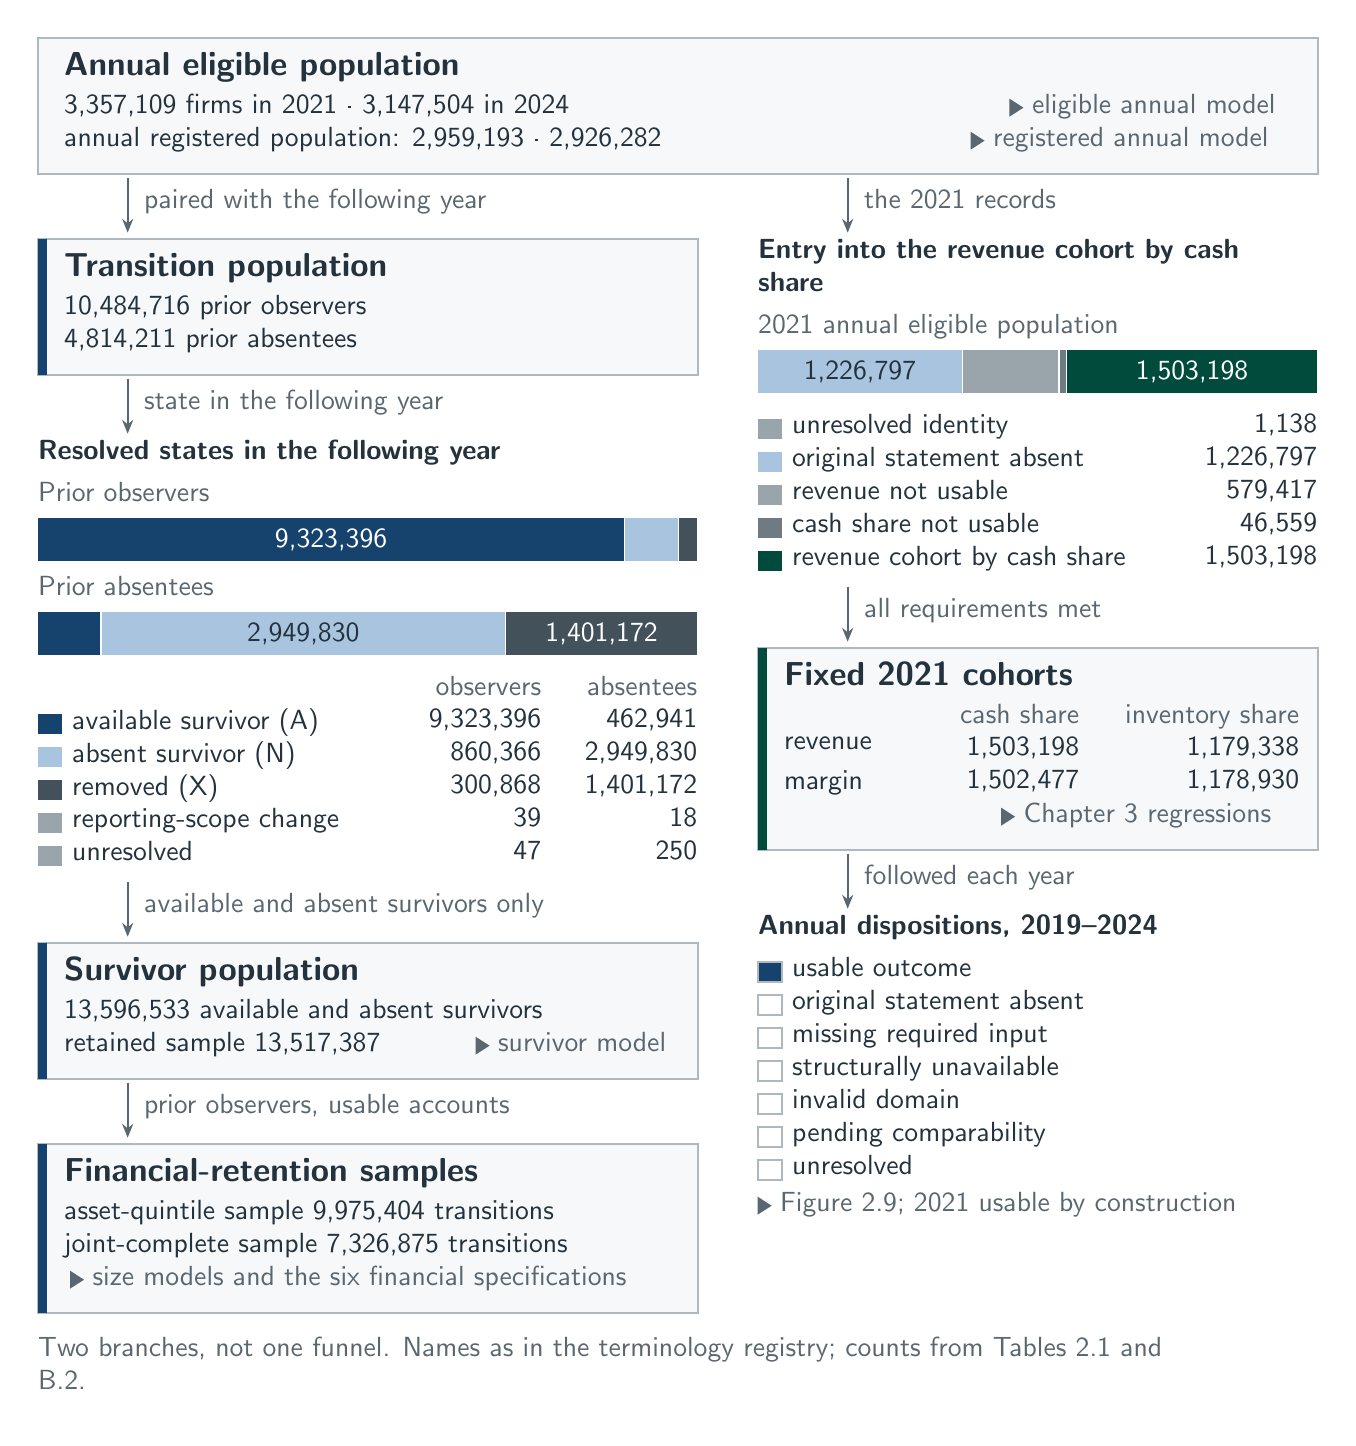
\begin{tikzpicture}[x=1in, y=-1in]\path (0,0) rectangle (6.5,6.9500);
\path[draw=rule, fill=boxfill, line width=0.6pt] (0.0500,0.0500) rectangle (6.4500,0.7300);
\node[anchor=north west, inner sep=0pt, text=ink, font=\bfseries\fontsize{11.5}{13}\selectfont] at (0.1800,0.1200) {Annual eligible population};
\node[anchor=north west, inner sep=0pt, text=ink] at (0.1800,0.3300) {3,357,109 firms in 2021 \textperiodcentered{} 3,147,504 in 2024};
\fill[muted] (4.9089,0.3550) -- (4.9789,0.4000) -- (4.9089,0.4450) -- cycle;
\node[anchor=north west, inner sep=0pt, text=muted] at (5.0189,0.3300) {eligible annual model};
\node[anchor=north west, inner sep=0pt, text=ink] at (0.1800,0.4950) {annual registered population: 2,959,193 \textperiodcentered{} 2,926,282};
\fill[muted] (4.7144,0.5200) -- (4.7844,0.5650) -- (4.7144,0.6100) -- cycle;
\node[anchor=north west, inner sep=0pt, text=muted] at (4.8244,0.4950) {registered annual model};
\draw[arrow] (0.5000,0.7500) -- (0.5000,1.0250);
\node[anchor=north west, inner sep=0pt, text=muted] at (0.5800,0.8050) {paired with the following year};
\path[draw=rule, fill=boxfill, line width=0.6pt] (0.0500,1.0550) rectangle (3.3500,1.7350);
\path[fill=navy] (0.0500,1.0550) rectangle (0.0950,1.7350);
\node[anchor=north west, inner sep=0pt, text=ink, font=\bfseries\fontsize{11.5}{13}\selectfont] at (0.1800,1.1250) {Transition population};
\node[anchor=north west, inner sep=0pt, text=ink] at (0.1800,1.3350) {10,484,716 prior observers};
\node[anchor=north west, inner sep=0pt, text=ink] at (0.1800,1.5000) {4,814,211 prior absentees};
\draw[arrow] (0.5000,1.7550) -- (0.5000,2.0300);
\node[anchor=north west, inner sep=0pt, text=muted] at (0.5800,1.8100) {state in the following year};
\node[anchor=north west, inner sep=0pt, text=ink, font=\bfseries] at (0.0500,2.0600) {Resolved states in the following year};
\node[anchor=north west, inner sep=0pt, text=muted] at (0.0500,2.2700) {Prior observers};
\path[fill=navy, draw=white, line width=0.5pt] (0.0500,2.4500) rectangle (2.9845,2.6700);
\node[anchor=center, inner sep=0pt, text=white] at (1.5172,2.5600) {9,323,396};
\path[fill=lightnavy, draw=white, line width=0.5pt] (2.9845,2.4500) rectangle (3.2553,2.6700);
\path[fill=darkgray, draw=white, line width=0.5pt] (3.2553,2.4500) rectangle (3.3500,2.6700);
\node[anchor=north west, inner sep=0pt, text=muted] at (0.0500,2.7400) {Prior absentees};
\path[fill=navy, draw=white, line width=0.5pt] (0.0500,2.9200) rectangle (0.3673,3.1400);
\path[fill=lightnavy, draw=white, line width=0.5pt] (0.3673,2.9200) rectangle (2.3894,3.1400);
\node[anchor=center, inner sep=0pt, text=ink] at (1.3783,3.0300) {2,949,830};
\path[fill=darkgray, draw=white, line width=0.5pt] (2.3894,2.9200) rectangle (3.3498,3.1400);
\node[anchor=center, inner sep=0pt, text=white] at (2.8696,3.0300) {1,401,172};
\node[anchor=north east, inner sep=0pt, text=muted] at (2.5700,3.2400) {observers};
\node[anchor=north east, inner sep=0pt, text=muted] at (3.3500,3.2400) {absentees};
\path[fill=navy] (0.0500,3.4300) rectangle (0.1700,3.5300);
\node[anchor=north west, inner sep=0pt, text=ink] at (0.2200,3.4050) {available survivor (A)};
\node[anchor=north east, inner sep=0pt, text=ink] at (2.5700,3.4050) {9,323,396};
\node[anchor=north east, inner sep=0pt, text=ink] at (3.3500,3.4050) {462,941};
\path[fill=lightnavy] (0.0500,3.5950) rectangle (0.1700,3.6950);
\node[anchor=north west, inner sep=0pt, text=ink] at (0.2200,3.5700) {absent survivor (N)};
\node[anchor=north east, inner sep=0pt, text=ink] at (2.5700,3.5700) {860,366};
\node[anchor=north east, inner sep=0pt, text=ink] at (3.3500,3.5700) {2,949,830};
\path[fill=darkgray] (0.0500,3.7600) rectangle (0.1700,3.8600);
\node[anchor=north west, inner sep=0pt, text=ink] at (0.2200,3.7350) {removed (X)};
\node[anchor=north east, inner sep=0pt, text=ink] at (2.5700,3.7350) {300,868};
\node[anchor=north east, inner sep=0pt, text=ink] at (3.3500,3.7350) {1,401,172};
\path[fill=gray] (0.0500,3.9250) rectangle (0.1700,4.0250);
\node[anchor=north west, inner sep=0pt, text=ink] at (0.2200,3.9000) {reporting-scope change};
\node[anchor=north east, inner sep=0pt, text=ink] at (2.5700,3.9000) {39};
\node[anchor=north east, inner sep=0pt, text=ink] at (3.3500,3.9000) {18};
\path[fill=gray] (0.0500,4.0900) rectangle (0.1700,4.1900);
\node[anchor=north west, inner sep=0pt, text=ink] at (0.2200,4.0650) {unresolved};
\node[anchor=north east, inner sep=0pt, text=ink] at (2.5700,4.0650) {47};
\node[anchor=north east, inner sep=0pt, text=ink] at (3.3500,4.0650) {250};
\draw[arrow] (0.5000,4.2700) -- (0.5000,4.5450);
\node[anchor=north west, inner sep=0pt, text=muted] at (0.5800,4.3250) {available and absent survivors only};
\path[draw=rule, fill=boxfill, line width=0.6pt] (0.0500,4.5750) rectangle (3.3500,5.2550);
\path[fill=navy] (0.0500,4.5750) rectangle (0.0950,5.2550);
\node[anchor=north west, inner sep=0pt, text=ink, font=\bfseries\fontsize{11.5}{13}\selectfont] at (0.1800,4.6450) {Survivor population};
\node[anchor=north west, inner sep=0pt, text=ink] at (0.1800,4.8550) {13,596,533 available and absent survivors};
\node[anchor=north west, inner sep=0pt, text=ink] at (0.1800,5.0200) {retained sample 13,517,387};
\fill[muted] (2.2394,5.0450) -- (2.3094,5.0900) -- (2.2394,5.1350) -- cycle;
\node[anchor=north west, inner sep=0pt, text=muted] at (2.3494,5.0200) {survivor model};
\draw[arrow] (0.5000,5.2750) -- (0.5000,5.5500);
\node[anchor=north west, inner sep=0pt, text=muted] at (0.5800,5.3300) {prior observers, usable accounts};
\path[draw=rule, fill=boxfill, line width=0.6pt] (0.0500,5.5800) rectangle (3.3500,6.4250);
\path[fill=navy] (0.0500,5.5800) rectangle (0.0950,6.4250);
\node[anchor=north west, inner sep=0pt, text=ink, font=\bfseries\fontsize{11.5}{13}\selectfont] at (0.1800,5.6500) {Financial-retention samples};
\node[anchor=north west, inner sep=0pt, text=ink] at (0.1800,5.8600) {asset-quintile sample 9,975,404 transitions};
\node[anchor=north west, inner sep=0pt, text=ink] at (0.1800,6.0250) {joint-complete sample 7,326,875 transitions};
\fill[muted] (0.2117,6.2150) -- (0.2817,6.2600) -- (0.2117,6.3050) -- cycle;
\node[anchor=north west, inner sep=0pt, text=muted] at (0.3217,6.1900) {size models and the six financial specifications};
\draw[arrow] (4.1000,0.7500) -- (4.1000,1.0250);
\node[anchor=north west, inner sep=0pt, text=muted] at (4.1800,0.8050) {the 2021 records};
\node[anchor=north west, inner sep=0pt, text=ink, font=\bfseries] at (3.6500,1.0550) {Entry into the revenue cohort by cash};
\node[anchor=north west, inner sep=0pt, text=ink, font=\bfseries] at (3.6500,1.2200) {share};
\node[anchor=north west, inner sep=0pt, text=muted] at (3.6500,1.4300) {2021 annual eligible population};
\path[fill=lightnavy, draw=white, line width=0.5pt] (3.6500,1.6100) rectangle (4.6732,1.8300);
\node[anchor=center, inner sep=0pt, text=ink] at (4.1616,1.7200) {1,226,797};
\path[fill=gray, draw=white, line width=0.5pt] (4.6732,1.6100) rectangle (5.1565,1.8300);
\path[fill=midgray, draw=white, line width=0.5pt] (5.1565,1.6100) rectangle (5.1953,1.8300);
\path[fill=green, draw=white, line width=0.5pt] (5.1953,1.6100) rectangle (6.4491,1.8300);
\node[anchor=center, inner sep=0pt, text=white] at (5.8222,1.7200) {1,503,198};
\path[fill=gray] (3.6500,1.9550) rectangle (3.7700,2.0550);
\node[anchor=north west, inner sep=0pt, text=ink] at (3.8200,1.9300) {unresolved identity};
\node[anchor=north east, inner sep=0pt, text=ink] at (6.4500,1.9300) {1,138};
\path[fill=lightnavy] (3.6500,2.1200) rectangle (3.7700,2.2200);
\node[anchor=north west, inner sep=0pt, text=ink] at (3.8200,2.0950) {original statement absent};
\node[anchor=north east, inner sep=0pt, text=ink] at (6.4500,2.0950) {1,226,797};
\path[fill=gray] (3.6500,2.2850) rectangle (3.7700,2.3850);
\node[anchor=north west, inner sep=0pt, text=ink] at (3.8200,2.2600) {revenue not usable};
\node[anchor=north east, inner sep=0pt, text=ink] at (6.4500,2.2600) {579,417};
\path[fill=midgray] (3.6500,2.4500) rectangle (3.7700,2.5500);
\node[anchor=north west, inner sep=0pt, text=ink] at (3.8200,2.4250) {cash share not usable};
\node[anchor=north east, inner sep=0pt, text=ink] at (6.4500,2.4250) {46,559};
\path[fill=green] (3.6500,2.6150) rectangle (3.7700,2.7150);
\node[anchor=north west, inner sep=0pt, text=ink] at (3.8200,2.5900) {revenue cohort by cash share};
\node[anchor=north east, inner sep=0pt, text=ink] at (6.4500,2.5900) {1,503,198};
\draw[arrow] (4.1000,2.7950) -- (4.1000,3.0700);
\node[anchor=north west, inner sep=0pt, text=muted] at (4.1800,2.8500) {all requirements met};
\path[draw=rule, fill=boxfill, line width=0.6pt] (3.6500,3.1000) rectangle (6.4500,4.1100);
\path[fill=green] (3.6500,3.1000) rectangle (3.6950,4.1100);
\node[anchor=north west, inner sep=0pt, text=ink, font=\bfseries\fontsize{11.5}{13}\selectfont] at (3.7800,3.1700) {Fixed 2021 cohorts};
\node[anchor=north east, inner sep=0pt, text=muted] at (5.2600,3.3800) {cash share};
\node[anchor=north east, inner sep=0pt, text=muted] at (6.3600,3.3800) {inventory share};
\node[anchor=north west, inner sep=0pt, text=ink] at (3.7800,3.5450) {revenue};
\node[anchor=north east, inner sep=0pt, text=ink] at (5.2600,3.5450) {1,503,198};
\node[anchor=north east, inner sep=0pt, text=ink] at (6.3600,3.5450) {1,179,338};
\node[anchor=north west, inner sep=0pt, text=ink] at (3.7800,3.7100) {margin};
\node[anchor=north east, inner sep=0pt, text=ink] at (5.2600,3.7100) {1,502,477};
\node[anchor=north east, inner sep=0pt, text=ink] at (6.3600,3.7100) {1,178,930};
\fill[muted] (4.8672,3.9000) -- (4.9372,3.9450) -- (4.8672,3.9900) -- cycle;
\node[anchor=north west, inner sep=0pt, text=muted] at (4.9772,3.8750) {Chapter 3 regressions};
\draw[arrow] (4.1000,4.1300) -- (4.1000,4.4050);
\node[anchor=north west, inner sep=0pt, text=muted] at (4.1800,4.1850) {followed each year};
\node[anchor=north west, inner sep=0pt, text=ink, font=\bfseries] at (3.6500,4.4350) {Annual dispositions, 2019--2024};
\path[fill=navy, draw=rule, line width=0.6pt] (3.6500,4.6700) rectangle (3.7700,4.7700);
\node[anchor=north west, inner sep=0pt, text=ink] at (3.8200,4.6450) {usable outcome};
\path[fill=white, draw=rule, line width=0.6pt] (3.6500,4.8350) rectangle (3.7700,4.9350);
\node[anchor=north west, inner sep=0pt, text=ink] at (3.8200,4.8100) {original statement absent};
\path[fill=white, draw=rule, line width=0.6pt] (3.6500,5.0000) rectangle (3.7700,5.1000);
\node[anchor=north west, inner sep=0pt, text=ink] at (3.8200,4.9750) {missing required input};
\path[fill=white, draw=rule, line width=0.6pt] (3.6500,5.1650) rectangle (3.7700,5.2650);
\node[anchor=north west, inner sep=0pt, text=ink] at (3.8200,5.1400) {structurally unavailable};
\path[fill=white, draw=rule, line width=0.6pt] (3.6500,5.3300) rectangle (3.7700,5.4300);
\node[anchor=north west, inner sep=0pt, text=ink] at (3.8200,5.3050) {invalid domain};
\path[fill=white, draw=rule, line width=0.6pt] (3.6500,5.4950) rectangle (3.7700,5.5950);
\node[anchor=north west, inner sep=0pt, text=ink] at (3.8200,5.4700) {pending comparability};
\path[fill=white, draw=rule, line width=0.6pt] (3.6500,5.6600) rectangle (3.7700,5.7600);
\node[anchor=north west, inner sep=0pt, text=ink] at (3.8200,5.6350) {unresolved};
\fill[muted] (3.6500,5.8450) -- (3.7200,5.8900) -- (3.6500,5.9350) -- cycle;
\node[anchor=north west, inner sep=0pt, text=muted] at (3.7600,5.8200) {Figure 2.9; 2021 usable by construction};
\node[anchor=north west, inner sep=0pt, text=muted] at (0.0500,6.5450) {Two branches, not one funnel. Names as in the terminology registry; counts from Tables 2.1 and};
\node[anchor=north west, inner sep=0pt, text=muted] at (0.0500,6.7100) {B.2.};
\end{tikzpicture}}
\pdfpagewidth=6.5in \pdfpageheight=6.9500in \hoffset=-1in \voffset=-1in \topskip=0pt \parskip=0pt
\shipout\vbox to \pdfpageheight{\hbox to 6.5in{\usebox\flowbox\hss}\vss}
\csname @@end\endcsname
